\section{Ứng dụng của tích phân}

\subsection{Diện tích, thể tích}

\subsubsection{Diện tích giữa hai đồ thị}
Nếu $f$ và $g$ là hai hàm số có tích phân trên $[a, b]$ và $f(x) \ge g(x)$ với mọi $x \in [a, b]$, thì \textbf{diện tích} của phần mặt phẳng nằm giữa đồ thị của $f$ và $g$ được định nghĩa là:
\[ A = \int_a^b [f(x) - g(x)] \dd x. \]
Chú ý rằng nếu $g(x) = 0$, công thức trên trở thành công thức tính diện tích miền dưới đồ thị hàm $f$ và trên trục $Ox$ như đã nêu trong Định nghĩa 5.1.5. TODO

\begin{example}
    Diện tích của hình chữ nhật $\{(x, y) \in \R^2 \mid a \le x \le b, c \le y \le d\}$ là diện tích của miền phẳng giới hạn bởi hai đường thẳng $y=d$ (đóng vai trò $f(x)$) và $y=c$ (đóng vai trò $g(x)$) trên đoạn $[a, b]$. Do đó, diện tích được tính bởi:
    \[ \int_a^b (d - c) \dd x = (d-c)x \bigg|_a^b = (d-c)(b-a). \]
\end{example}

\begin{example}
    Tìm diện tích của miền được giới hạn bởi hai parabol $y = x^2$ và $y = 2x - x^2$.
\end{example}
\begin{solution}
    Trước hết, ta tìm giao điểm của hai đường cong bằng cách giải phương trình:
    \[ x^2 = 2x - x^2 \implies 2x^2 - 2x = 0 \implies 2x(x-1) = 0. \]
    Vậy hai đồ thị cắt nhau tại $x=0$ và $x=1$. Trên đoạn $[0, 1]$, ta kiểm tra thấy $2x - x^2 \ge x^2$ (ví dụ tại $x=0.5$, ta có $0.75 > 0.25$). Do đó, diện tích của miền nằm giữa hai đồ thị là:
    \begin{align*}
        A &= \int_0^1 \left[(2x - x^2) - x^2\right] \dd x \\
        &= \int_0^1 (2x - 2x^2) \dd x \\
        &= \left[x^2 - \dfrac{2}{3}x^3\right]_0^1 \\
        &= \left(1 - \dfrac{2}{3}\right) - 0 = \dfrac{1}{3}.
    \end{align*}
\end{solution}

\subsubsection{Thể tích}
Nếu một vật thể trong không gian $\R^3$ có diện tích mặt cắt (tiết diện) vuông góc với trục $Ox$ tại một điểm $x \in [a, b]$ là $A(x)$, ta có thể định nghĩa \textbf{thể tích} của vật thể đó là:
\begin{importantbox}
    \[ V = \int_a^b A(x) \dd x. \]
\end{importantbox}

\begin{figure}[H]
    \centering
    \begin{minipage}{0.45\textwidth}
        \centering
        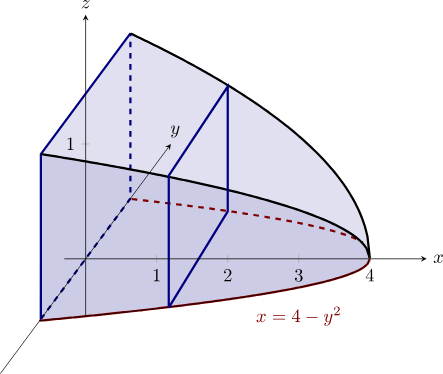
\includegraphics[width=\textwidth]{figures/accumulated_cross_sections_1.png}
    \end{minipage}
    \vspace{1em}
    \begin{minipage}{0.45\textwidth}
        \centering
        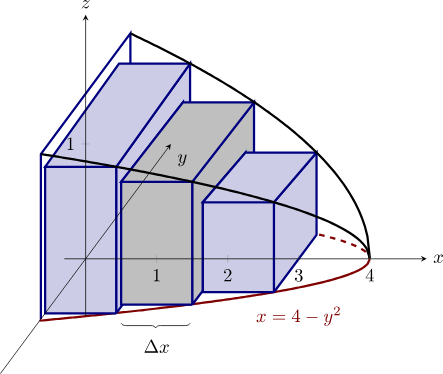
\includegraphics[width=\textwidth]{figures/accumulated_cross_sections_2.png}
    \end{minipage}
    \label{fig:volume-cross-section}
    \caption{Thể tích của khối qua diện tích mặt cắt\footnotemark}
\end{figure}
\footnotetext{nguồn \href{https://ximera.osu.edu/csccmathematics/calculus2/accumulatedCrossSections/digInAccumulatedCrossSections}{XIMERA}}

Định nghĩa này nói rằng thể tích của khối bằng ``tổng'' của diện tích tất cả các mặt cắt song song. Phương pháp này còn được gọi là \textbf{phương pháp cắt lớp}.

\begin{example}
    Thể tích của một quả cầu bán kính $R$ là $V = \dfrac{4}{3}\pi R^3$.
\end{example}
\begin{solution}
    Xét một quả cầu có tâm tại gốc tọa độ $O$ và bán kính $R$. Một lát cắt vuông góc với trục $Ox$ tại vị trí $x$ là một hình tròn. Bán kính $r$ của hình tròn này thỏa mãn $r^2 + x^2 = R^2$, suy ra $r = \sqrt{R^2 - x^2}$.
    Diện tích của mặt cắt này là:
    \[ A(x) = \pi r^2 = \pi (\sqrt{R^2 - x^2})^2 = \pi(R^2 - x^2). \]
    Do đó, thể tích của quả cầu được tính bằng cách lấy tích phân của $A(x)$ từ $-R$ đến $R$:
    \begin{align*}
        V &= \int_{-R}^R \pi(R^2 - x^2) \dd x \\
        &= \pi \left[ R^2x - \dfrac{x^3}{3} \right]_{-R}^R \\
        &= \pi \left[ \left(R^3 - \dfrac{R^3}{3}\right) - \left(-R^3 - \dfrac{(-R)^3}{3}\right) \right] \\
        &= \pi \left[ \dfrac{2R^3}{3} - \left(-\dfrac{2R^3}{3}\right) \right] = \dfrac{4}{3}\pi R^3.
    \end{align*}
\end{solution}

\begin{example}
    Một \textbf{khối tròn xoay} được tạo ra khi quay một miền phẳng quanh một đường thẳng. Giả sử $f(x) \ge 0$ trên $[a, b]$, xét khối tròn xoay thu được khi quay miền giới hạn bởi đồ thị của $f$, trục $Ox$, và hai đường thẳng $x=a, x=b$ quanh trục $Ox$. Mỗi lát cắt vuông góc tại $x$ của khối này là một hình tròn có bán kính là $f(x)$. Do đó, diện tích mặt cắt là $A(x) = \pi [f(x)]^2$. Thể tích của khối tròn xoay này là:
    \[ V = \pi \int_a^b [f(x)]^2 \dd x. \]
\end{example}

%% Ghi chú: Ví dụ gốc (5.4.5) đã được thay đổi để tránh sao chép.
\begin{example}
    Khi xoay miền giới hạn bởi đường $y = \sqrt{x}$ và trục $Ox$ trên đoạn $[0, 4]$ quanh trục $Ox$, ta được một vật thể có hình dạng paraboloid. Thể tích của khối này là:
    \[ V = \pi \int_0^4 (\sqrt{x})^2 \dd x = \pi \int_0^4 x \dd x = \pi \left[\dfrac{x^2}{2}\right]_0^4 = 8\pi. \]
\end{example}

Đề tài về diện tích và thể tích sẽ được khảo sát một cách hệ thống và tổng quát hơn trong môn Vi tích phân 2 [Bmgt2, Chương 2].

\subsection{Giá trị trung bình}

Nếu tại các điểm rời rạc $x_1, x_2, \dots, x_n$ ta có các giá trị tương ứng $f(x_1), f(x_2), \dots, f(x_n)$, thì giá trị trung bình của các giá trị này được tính bằng công thức $\dfrac{1}{n}\sum_{i=1}^n f(x_i)$. Trong trường hợp miền xác định là một khoảng liên tục $[a, b]$, ta mở rộng khái niệm này bằng cách thay phép lấy tổng bằng phép lấy tích phân.

\begin{definition}
    \textbf{Giá trị trung bình} của một hàm số $f$ khả tích trên đoạn $[a, b]$ được định nghĩa là:
    \begin{importantbox}
        \[ f_{\text{tb}} = \dfrac{1}{b-a} \int_a^b f(x) \dd x. \]
    \end{importantbox}
\end{definition}

Giá trị trung bình của một hàm số trên một miền xác định có thể được hiểu là ``tổng'' các giá trị của hàm chia cho ``độ dài'' của miền đó.

Ta có thể giải thích chi tiết hơn như sau. Chia đoạn $[a, b]$ thành $n$ đoạn con có cùng chiều dài $\Delta x = \dfrac{b-a}{n}$, với các điểm chia $a = x_0, x_1, \dots, x_n = b$. Lấy các điểm mẫu $x_i^* \in [x_{i-1}, x_i]$. Giá trị trung bình của hàm tại các điểm mẫu này là:
\[ \dfrac{f(x_1^*) + f(x_2^*) + \dots + f(x_n^*)}{n}. \]
Ta biến đổi biểu thức này:
\begin{align*}
    \dfrac{1}{n} \sum_{i=1}^n f(x_i^*) &= \dfrac{1}{b-a} \cdot \dfrac{b-a}{n} \sum_{i=1}^n f(x_i^*) \\
    &= \dfrac{1}{b-a} \sum_{i=1}^n f(x_i^*) \Delta x.
\end{align*}
Số hạng $\sum_{i=1}^n f(x_i^*) \Delta x$ chính là một tổng Riemann của $f$. Khi cho $n \to \infty$, tổng Riemann này tiến tới tích phân $\int_a^b f(x) \dd x$. Do đó, ta đi đến định nghĩa về giá trị trung bình của hàm số.

%% Ghi chú: Ví dụ gốc 5.4.6 đã được thay đổi. Mô hình nhiệt độ được thay bằng mô hình mực nước thủy triều.
%% Các hằng số và hàm lượng giác đã được điều chỉnh.
\begin{example}
    Mực nước (tính bằng mét) tại một bến cảng trong một ngày được mô hình hóa bởi hàm số $L(t) = 5 + 2\cos\left(\dfrac{\pi t}{6}\right)$, trong đó $t$ là số giờ tính từ 6 giờ sáng. Hãy tìm mực nước trung bình từ 6 giờ sáng đến 12 giờ trưa.
\end{example}
\begin{solution}
    Khoảng thời gian từ 6 giờ sáng đến 12 giờ trưa tương ứng với $t$ từ $0$ đến $6$. Giá trị trung bình của $L(t)$ trên đoạn $[0, 6]$ là:
    \begin{align*}
        L_{\text{tb}} &= \dfrac{1}{6-0} \int_0^6 \left(5 + 2\cos\left(\dfrac{\pi t}{6}\right)\right) \dd t \\
        &= \dfrac{1}{6} \left[ 5t + 2 \cdot \dfrac{6}{\pi}\sin\left(\dfrac{\pi t}{6}\right) \right]_0^6 \\
        &= \dfrac{1}{6} \left[ \left(30 + \dfrac{12}{\pi}\sin(\pi)\right) - \left(0 + \dfrac{12}{\pi}\sin(0)\right) \right] \\
        &= \dfrac{1}{6} [30] = 5.
    \end{align*}
    Vậy, mực nước trung bình trong khoảng thời gian đó là 5 mét.
\end{solution}

%% Ghi chú: Ví dụ gốc 5.4.7 là một khái niệm cơ bản nên được giữ lại, nhưng được diễn giải lại để đảm bảo tính độc đáo.
\begin{example}[Vận tốc trung bình]
    Xét một vật di chuyển trên một đường thẳng. Vị trí của vật tại thời điểm $t$ được cho bởi hàm số $x(t)$. Vận tốc tức thời $v(t)$ là đạo hàm của vị trí theo thời gian, tức là $v(t) = x'(t)$. Chú ý rằng \textbf{vận tốc (velocity)} có thể mang giá trị âm (chuyển động theo chiều ngược lại), khác với \textbf{tốc độ (speed)} là độ lớn của vận tốc và luôn không âm.
    
    Giả sử vật di chuyển trong khoảng thời gian từ $a$ đến $b$. Giá trị trung bình của vận tốc trong khoảng thời gian này là:
    \[ v_{\text{tb}} = \dfrac{1}{b-a} \int_a^b v(t) \dd t = \dfrac{1}{b-a} \int_a^b x'(t) \dd t. \]
    Theo Công thức Newton-Leibniz, ta có:
    \[ v_{\text{tb}} = \dfrac{1}{b-a} \left[ x(t) \right]_a^b = \dfrac{x(b) - x(a)}{b-a}. \]
    Kết quả này chính là định nghĩa quen thuộc của vận tốc trung bình: độ dời chia cho khoảng thời gian. Cần lưu ý rằng, vận tốc trung bình có thể khác với tốc độ trung bình (là tổng quãng đường đi được chia cho khoảng thời gian), đặc biệt là khi vật đổi chiều chuyển động.
\end{example}

\subsection{Một số ứng dụng trong khoa học}
Một trong những ý nghĩa chính của tích phân là phép tính tổng, vì vậy mỗi khi trong khoa học kỹ thuật có nhu cầu tính tổng của vô hạn các giá trị thì tích phân có thể xuất hiện. Ở đây, ta sẽ nghiên cứu các ứng dụng chủ yếu qua các ví dụ và bài toán. Người đọc có thể tham khảo thêm nhiều ví dụ ứng dụng khác trong các tài liệu như [Ste16]. TODO

\begin{example}[Mạch máu]
    Luật Poiseuille mô tả tốc độ của dòng máu chảy trong một mạch máu có dạng hình trụ:
    \[ v(r) = \dfrac{P}{4\eta l}(R^2 - r^2) \]
    trong đó $v$ là vận tốc dòng máu tại khoảng cách $r$ tính từ trục tâm, $R$ là bán kính của mạch máu, $l$ là độ dài mạch máu, $P$ là chênh lệch áp suất giữa hai đầu mạch máu, và $\eta$ là độ nhớt của máu. Ta muốn tính tổng lưu lượng máu (thể tích máu chảy qua một mặt cắt của mạch máu trong một đơn vị thời gian).
    
    Thể tích máu chảy qua một vòng xuyến mỏng có bán kính $r$ và độ dày $\dd r$ trong một đơn vị thời gian xấp xỉ bằng $v(r) \times (\text{diện tích vòng xuyến}) \approx v(r) \cdot 2\pi r \dd r$.
    Tổng lưu lượng máu trong toàn bộ mạch máu là tích phân của đại lượng này theo bán kính từ $0$ đến $R$:
    \begin{align*}
        Q = \int_0^R v(r) 2\pi r \dd r &= \int_0^R \dfrac{P}{4\eta l}(R^2 - r^2) 2\pi r \dd r \\
        &= \dfrac{2\pi P}{4\eta l} \int_0^R (R^2r - r^3) \dd r \\
        &= \dfrac{\pi P}{2\eta l} \left[ R^2\dfrac{r^2}{2} - \dfrac{r^4}{4} \right]_0^R \\
        &= \dfrac{\pi P}{2\eta l} \left( \dfrac{R^4}{2} - \dfrac{R^4}{4} \right) = \dfrac{\pi P R^4}{8\eta l}.
    \end{align*}
\end{example}

\begin{example}[Thủy lực]
    Một cửa cống hình chữ nhật, thẳng đứng, có chiều cao 15 mét và chiều rộng 40 mét. Tính tổng lực (áp lực) của nước tác động lên cửa cống nếu mực nước cao 10 mét.
\end{example}
\begin{solution}
    Áp lực của một chất lỏng tĩnh có mật độ khối lượng $\rho$ ở độ sâu $d$ được cho bởi công thức $P = \rho g d$, trong đó $g$ là gia tốc trọng trường. Nguyên lý Pascal cho biết áp lực tại một điểm trong chất lỏng tĩnh là như nhau theo mọi hướng.
    
    Ta đặt một hệ tọa độ lên mặt phẳng của cửa cống, với gốc tọa độ ở đáy cống, trục $y$ hướng thẳng đứng lên trên. Mực nước ở độ cao $y=10$.
        
    \begin{figure}[H]
        \centering
        \begin{tikzpicture}
            % Dam
            \draw[fill=gray!30] (0,0) rectangle (6,15/2.5);
            % Water
            \draw[fill=blue!20] (0,0) rectangle (6,10/2.5);
            \node at (3,12/2.5) [above] {Mực nước};
            
            % Coordinate system
            \draw[->] (-1,0) -- (7,0) node[below] {$x (m)$};
            \draw[->] (0,-1) -- (0,7) node[left] {$y (m)$};
            \node at (6,0) [below] {40};
            \node at (0,15/2.5) [left] {15};
            \node at (0,10/2.5) [left] {10};
            
            % A thin strip
            \draw[dashed, red] (0, 5/2.5) -- (6, 5/2.5);
            \node at (-0.5, 5/2.5) {$y$};
            \draw[<->] (6.2, 5/2.5) -- (6.2, 10/2.5);
            \node at (7, 7.5/2.5) {$10-y$};
        \end{tikzpicture}
        \caption{Sơ đồ tính áp lực nước lên cửa cống.}
    \end{figure}
    
    Xét một dải mỏng nằm ngang của cửa cống ở độ cao $y$ với độ dày $\dd y$. Độ sâu của dải này là $10-y$. Áp lực nước tại độ sâu này là $P(y) = \rho g (10-y)$.
    Diện tích của dải mỏng là $dA = 40 \dd y$. Lực tác động lên dải này là $\dd F = P(y) \dd A = \rho g (10-y) (40 \dd y)$.
    Tổng lực tác động lên toàn bộ phần ngập nước của cửa cống là tích phân của $\dd F$ từ $y=0$ đến $y=10$. Với $\rho_{\text{nước}} \approx 1000$ kg/m$^3$ và $g \approx 9,8$ m/s$^2$:
    \begin{align*}
        F = \int_0^{10} 40 \rho g (10-y) \dd y &= 40 \cdot 1000 \cdot 9,8 \int_0^{10} (10-y) \dd y \\
        &= 392000 \left[ 10y - \dfrac{y^2}{2} \right]_0^{10} \\
        &= 392000 \left( 100 - \dfrac{100}{2} \right) \\
        &= 392000 \cdot 50 = 19,6 \cdot 10^6 \text{ (N)}.
    \end{align*}
    Đơn vị của lực là Newton (N).
\end{solution}

\subsubsection{Hàm mật độ}
Nếu tại mỗi điểm $x_i$ ($1 \le i \le n$) có một đại lượng tương ứng là $f(x_i)$, thì tổng giá trị của đại lượng đó là $\sum_{i=1}^n f(x_i)$. Khi tập hợp các điểm $D$ là một khoảng liên tục, hàm $f$ từ $D$ vào $\R$ được gọi là \textbf{hàm mật độ} của đại lượng, và tổng giá trị của đại lượng là tích phân $\int_D f(x) \dd x$.
Trong vật lý, khối lượng của một vật là tích phân của hàm mật độ khối lượng trên miền không gian mà vật chiếm giữ.

\begin{example}
    Tìm khối lượng của một sợi dây dài 1 mét có mật độ khối lượng tuyến tính (khối lượng trên một đơn vị chiều dài) là $\rho(x) = 1 + \sin(\pi x)$ (kg/m), với $x$ là khoảng cách từ một đầu của sợi dây.
\end{example}
\begin{solution}
    Khối lượng của sợi dây bằng tích phân của hàm mật độ khối lượng trên suốt chiều dài của nó:
    \begin{align*}
        M = \int_0^1 \rho(x) \dd x &= \int_0^1 (1 + \sin(\pi x)) \dd x \\
        &= \left[ x - \dfrac{1}{\pi}\cos(\pi x) \right]_0^1 \\
        &= \left( 1 - \dfrac{1}{\pi}\cos(\pi) \right) - \left( 0 - \dfrac{1}{\pi}\cos(0) \right) \\
        &= \left( 1 + \dfrac{1}{\pi} \right) - \left( -\dfrac{1}{\pi} \right) = 1 + \dfrac{2}{\pi} \approx 1,637 \text{ (kg)}.
    \end{align*}
\end{solution}

\subsubsection{Công}
Giả sử một vật di chuyển dưới tác dụng của một lực. \textbf{Công} của lực là một khái niệm vật lý đại diện cho năng lượng mà lực truyền cho vật trong quá trình di chuyển.
Nếu một vật di chuyển một quãng đường $d$ trên một đường thẳng dưới tác dụng của một lực không đổi $F$ cùng chiều chuyển động, công sinh ra được định nghĩa là $W = F \cdot d$.

Bây giờ, xét trường hợp tổng quát hơn, khi lực $F$ có thể thay đổi độ lớn theo vị trí, nhưng vẫn cùng phương với chuyển động. Đặt một trục tọa độ dọc theo phương chuyển động. Độ lớn của lực tác dụng lên vật tại vị trí $x$ là $F(x)$. Giả sử vật di chuyển từ vị trí $x=a$ đến vị trí $x=b$. Công của lực $F$ là ``tổng'' của các giá trị $F(x)$ trên suốt quãng đường, được cho bởi tích phân:
\[ W = \int_a^b F(x) \dd x. \]

\begin{example}[Định lý công-động năng]
    Giả sử một vật có khối lượng $m$ di chuyển dưới tác dụng của một tổng hợp lực $F$. Vị trí của vật tại thời điểm $t$ là $x(t)$, vận tốc là $v(t) = x'(t)$, và gia tốc là $a(t) = v'(t) = x''(t)$. Giả sử vật di chuyển từ $x(t_0) = a$ đến $x(t_1) = b$. \textbf{Động năng} (năng lượng do chuyển động) của vật là $K(t) = \dfrac{1}{2}mv(t)^2 = \dfrac{1}{2}m[x'(t)]^2$.
    
    Theo định luật II Newton: $F = ma = mx''$. Do đó, công của lực $F$ khi vật di chuyển từ $a$ đến $b$ là:
    \[ W = \int_a^b F(x) \dd x = \int_{t_0}^{t_1} F(x(t)) x'(t) \dd t = \int_{t_0}^{t_1} m x''(t) x'(t) \dd t. \]
    Sử dụng hằng đẳng thức $\deriv{}{t} [x'(t)]^2 = 2x'(t)x''(t)$, ta biến đổi:
    \begin{align*}
        W = \int_{t_0}^{t_1} m \cdot \dfrac{1}{2} \deriv{}{t}[x'(t)]^2 \dd t &= \dfrac{1}{2}m \int_{t_0}^{t_1} \deriv{}{t}[x'(t)]^2 \dd t \\
        &= \dfrac{1}{2}m [x'(t)]^2 \bigg|_{t_0}^{t_1} \\
        &= \dfrac{1}{2}m[x'(t_1)]^2 - \dfrac{1}{2}m[x'(t_0)]^2 = K(t_1) - K(t_0).
    \end{align*}
    Vậy, ta thu được bằng phương pháp toán học một định luật vật lý quan trọng: \textbf{công của ngoại lực tác dụng lên vật bằng độ biến thiên động năng của vật đó}.
\end{example}

\subsection{Xác suất}

Trong lý thuyết xác suất, một \textbf{biến ngẫu nhiên} $X$ là một ánh xạ từ một tập hợp các sự kiện vào tập hợp các số thực.

\subsubsection{Biến ngẫu nhiên rời rạc}
Trong trường hợp tập giá trị $D$ của $X$ là hữu hạn, ta nói $X$ là một \textbf{biến ngẫu nhiên rời rạc}. Với mỗi giá trị $x \in D$, có một số thực $0 \le p(x) \le 1$ là xác suất để $X$ có giá trị $x$ (giá trị 1 tương ứng với 100\%). Hàm $p$ được gọi là \textbf{hàm xác suất} của biến ngẫu nhiên $X$. Xác suất để $X$ có giá trị nằm trong một tập con $C \subset D$ được cho bởi:
\[ P(X \in C) = \sum_{x \in C} p(x). \]
Một hệ quả là tổng xác suất trên toàn bộ không gian mẫu phải bằng 1, tức là $\sum_{x \in D} p(x) = 1$. \textbf{Giá trị trung bình} (mean) hay \textbf{kỳ vọng} (expectation) của $X$ được cho bởi:
\[ E[X] = \sum_{x \in D} x \cdot p(x). \]

\begin{example}
    Xét một trò chơi tung đồng xu công bằng như sau: Người chơi trả 5 nghìn đồng cho mỗi lần tung. Nếu mặt ngửa xuất hiện, người chơi nhận được 8 nghìn đồng. Nếu mặt sấp xuất hiện, người chơi không nhận được gì. Hỏi trung bình người chơi sẽ lãi hay lỗ?
\end{example}
\begin{solution}
    Gọi $X$ là số tiền người chơi nhận được. $X$ có thể nhận hai giá trị: $8$ (nếu ngửa) và $0$ (nếu sấp). Vì đồng xu công bằng, xác suất của mỗi kết quả là $1/2$.
    Hàm xác suất là $p(8) = 1/2$ và $p(0) = 1/2$.
    Kỳ vọng của số tiền nhận được là:
    \[ E[X] = 8 \cdot p(8) + 0 \cdot p(0) = 8 \cdot \dfrac{1}{2} + 0 \cdot \dfrac{1}{2} = 4. \]
    Kỳ vọng số tiền nhận được là 4 nghìn đồng, trong khi chi phí mỗi lần chơi là 5 nghìn đồng. Như vậy, về lâu dài, trung bình mỗi lần chơi người chơi sẽ lỗ 1 nghìn đồng.
\end{solution}

\subsubsection{Biến ngẫu nhiên liên tục}
Trong trường hợp tập giá trị của biến ngẫu nhiên $X$ là một khoảng số thực $D$ (có thể là $(-\infty, \infty)$), ta nói $X$ là một \textbf{biến ngẫu nhiên liên tục}. Tương tự với trường hợp rời rạc, có một \textbf{hàm mật độ xác suất} (probability density function - PDF) $f$ xác định trên $D$ sao cho $f(x) \ge 0$ và xác suất để $X$ có giá trị trong một khoảng $[c, d] \subset D$ được tính bằng tích phân:
\[ P(c \le X \le d) = \int_c^d f(x) \dd x. \]
Hàm mật độ xác suất phải thỏa mãn điều kiện chuẩn hóa:
\[ \int_D f(x) \dd x = 1. \]
Tương tự, kỳ vọng của biến ngẫu nhiên liên tục $X$ được tính bằng tích phân:
\[ E[X] = \int_D x f(x) \dd x. \]

%% Ghi chú: Ví dụ gốc 5.4.13 đã được thay đổi. Mô hình tuổi thọ của bóng đèn được sử dụng thay cho sản phẩm.
\begin{example}
    Gọi $T$ là biến ngẫu nhiên biểu thị tuổi thọ của một loại bóng đèn LED (tính bằng nghìn giờ). Giả sử hàm mật độ xác suất của $T$ là $f(t) = 0.05e^{-0.05t}$ với $t \ge 0$.
\end{example}
\begin{solution}
    (a) Xác suất một bóng đèn hỏng trong vòng 10,000 giờ đầu tiên (tức là $0 \le T \le 10$) là:
    \[ P(0 \le T \le 10) = \int_0^{10} 0.05e^{-0.05t} \dd t = \left[-e^{-0.05t}\right]_0^{10} = -e^{-0.5} - (-e^0) = 1 - e^{-0.5} \approx 0.393. \]
    Vậy có khoảng 39.3\% khả năng bóng đèn sẽ hỏng trong 10,000 giờ đầu.

    (b) Tuổi thọ trung bình (kỳ vọng) của bóng đèn là:
    \[ E[T] = \int_0^\infty t \cdot f(t) \dd t = \int_0^\infty 0.05t e^{-0.05t} \dd t. \]
    Ta tính tích phân từng phần với $u = t$ và $\dd v = 0.05e^{-0.05t} \dd t$. Suy ra $\dd u = \dd t$ và $v = -e^{-0.05t}$.
    \begin{align*}
        E[T] &= \lim_{h \to \infty} \left( [-te^{-0.05t}]_0^h - \int_0^h (-e^{-0.05t}) \dd t \right) \\
        &= \lim_{h \to \infty} \left( -he^{-0.05h} - \left[ \dfrac{1}{0.05}e^{-0.05t} \right]_0^h \right) \\
        &= \lim_{h \to \infty} \left( -he^{-0.05h} - 20(e^{-0.05h} - 1) \right).
    \end{align*}
    Sử dụng quy tắc L'Hôpital, $\lim_{h \to \infty} he^{-0.05h} = \lim_{h \to \infty} \frac{h}{e^{0.05h}} = 0$.
    Do đó, $E[T] = 0 - 20(0 - 1) = 20$.
    Vậy, tuổi thọ trung bình của bóng đèn là 20,000 giờ.
\end{solution}

\begin{example}[Phân bố chuẩn]
    Nhiều hiện tượng ngẫu nhiên trong tự nhiên và xã hội được mô hình hóa bằng \textbf{phân bố chuẩn} (normal distribution), với hàm mật độ xác suất có dạng:
    \[ f(x) = \dfrac{1}{\sigma\sqrt{2\pi}} e^{-\frac{(x-\mu)^2}{2\sigma^2}}. \]
    Ở đây, $\mu$ là giá trị trung bình (kỳ vọng) và $\sigma$ là \textbf{độ lệch chuẩn} (standard deviation), đo lường mức độ phân tán của các giá trị. Đồ thị của hàm này có dạng hình chuông đặc trưng.
        Việc đây thực sự là một hàm mật độ xác suất là hệ quả của một công thức tích phân nổi tiếng:
    \[ \int_{-\infty}^\infty e^{-x^2} \dd x = \sqrt{\pi}. \]
    Công thức quan trọng này có thể được chứng minh bằng cách sử dụng tích phân của hàm hai biến trong [Bmgt2, Chương 2].
    
    Môn học Xác suất Thống kê sẽ thảo luận chi tiết hơn về chủ đề này ([NTNM22], [Ros20]).
\end{example}

\subsection{Bài tập}
\subsubsection{Diện tích, thể tích}

\begin{exercise}
    Tính diện tích của miền được giới hạn bởi các đường cong đã cho.
    \begin{enumerate}[label=(\alph*)]
        \item $y = x^2 - 2x$ và $y = x+4$.
        \item $y = x^3 - x$ và $y = 3x$.
        \item $y = \sin x$, $y = \cos x$, $x=0$, và $x=\pi/2$.
        \item $y = (x-2)^2$ và $y=x$.
        \item $y = |x|$ và $y = x^2 - 2$.
        \item $x = 2y^2$ và $x = 4+y^2$.
        \item $y = 1/x$, $y=x^2$, $y=0$, $x=e$.
        \item $y = e^x$, $y=e^{-x}$, và $x=1$.
        \item $y = x^4 - 4x^2 + 4$ và $y=x^2$.
        \item $y=x\sqrt{x-1}$ và $y=2\sqrt{x-1}$.
        \item $x=y^3-y$ và $x=0$.
        \item $y = \dfrac{1}{1+x^2}$ và $y = \dfrac{1}{2}|x|$.
    \end{enumerate}
\end{exercise}

\begin{exercise}
    Sử dụng chương trình máy tính (tham khảo Hướng dẫn ở trang 187) để vẽ đồ thị và tìm diện tích (xấp xỉ) của miền được giới hạn bởi các đường cong:
    \begin{enumerate}[label=(\alph*)]
        \item $y = x^5 - 6x^3 + 4x$ và $y=x$.
        \item $y = x \cos(x^2)$ và $y = x^3 - x$.
    \end{enumerate}
\end{exercise}

\begin{exercise}
    Một máy chụp cắt lớp vi tính (CAT scan) tạo ra các hình ảnh cắt ngang của một cơ quan trong cơ thể. Giả sử máy quét chụp các lát cắt của một lá gan, với các lát cắt cách đều nhau 1 cm. Cho biết chiều dài của lá gan là 10 cm và diện tích của các mặt cắt ngang (đơn vị cm$^2$) tại các vị trí $x=0, 1, ..., 10$ lần lượt là: 0, 25, 60, 85, 105, 110, 100, 80, 50, 15, 0. Hãy dùng tổng Riemann (ví dụ: quy tắc hình thang hoặc quy tắc trung điểm) để ước tính thể tích của lá gan.
\end{exercise}

\begin{exercise}
    Tìm thể tích của khối tròn xoay được tạo thành khi quay miền được giới hạn bởi các đường cong cho trước quanh trục đã chỉ định, Hình~\ref{fig:volumn_solid_revolution}.
    
    % Placeholder for the image of the solid of revolution
    \begin{figure}[H]
        \centering
        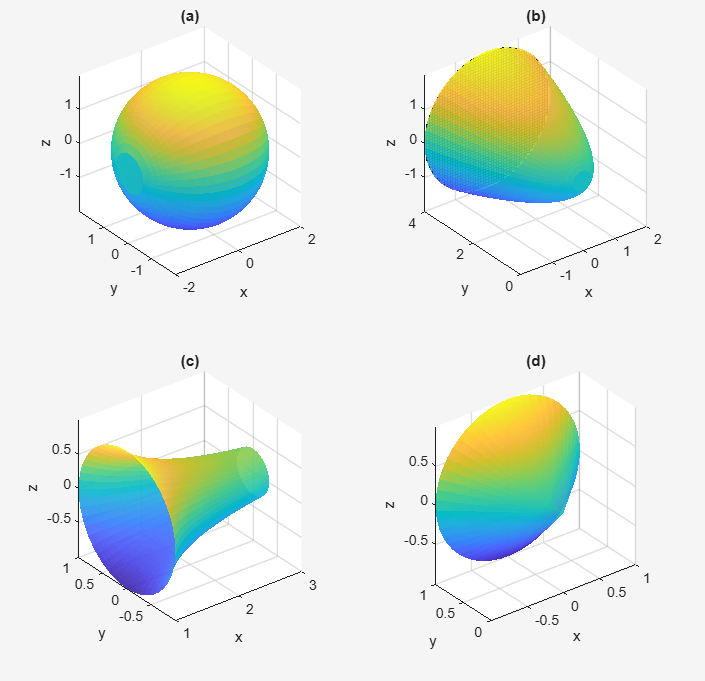
\includegraphics[width=0.8\linewidth]{figures/volumn_solid_revolution.png}
        \caption{Thể tích của các khối tạo bởi đường cong quay quanh trục}
        \label{fig:volumn_solid_revolution}
    \end{figure}
    
    \begin{enumerate}[label=(\alph*)]
        \item $y = \sqrt{4-x^2}$, $y=0$, quanh trục $x$.
        \item $y = x^2$, $y=4$, $x=0$, quanh trục $y$.
        \item $y = 1/x$, $x=1$, $x=3$, $y=0$, quanh trục $x$.
        \item $y = x$, $y = \sqrt{x}$, quanh trục $y$.
    \end{enumerate}
\end{exercise}

\begin{exercise}
    Tìm thể tích của khối được tạo bằng cách xoay miền bao bởi đồ thị của hàm số $f(x) = x(x-1)^2$ và trục $x$ quanh trục $y$.
\end{exercise}

\begin{exercise}
    Chứng tỏ rằng ``sừng Gabriel'', là khối không gian nhận được bằng cách xoay quanh trục $x$ phần mặt phẳng bên dưới đồ thị của hàm $y = 1/x$ bên trên trục $x$ với $x \ge 1$, có thể tích hữu hạn nhưng diện tích bề mặt là vô hạn.
\end{exercise}

\begin{exercise}
    Tính thể tích của các khối rắn $S$ được mô tả sau đây.
    \begin{enumerate}[label=(\alph*)]
        \item Một khối nón thẳng đứng có chiều cao $h$ và bán kính đáy $r$.
        \item Một khối chóp cụt có chiều cao $h$, đáy dưới là hình vuông cạnh $B$, và đáy trên là hình vuông cạnh $b$.
        \item Một nắp chỏm cầu có chiều cao $h$ được cắt từ một quả cầu có bán kính $r$.
        \item Một khối chóp có chiều cao $h$ và đáy là một tam giác đều cạnh $a$.
        \item Một khối chóp có chiều cao $h$ và đáy là một hình chữ nhật có kích thước $L \times W$.
        \item Một cái nêm được cắt ra từ một khối trụ (bán kính 5) bởi một mặt phẳng đi qua đường kính của đáy và một mặt phẳng khác nghiêng một góc 45 độ so với đáy.
        \item Một khối có đáy là hình tròn $x^2+y^2=4$. Các mặt cắt vuông góc với trục $x$ là các tam giác vuông cân có cạnh góc vuông nằm trên đáy.
    \end{enumerate}
\end{exercise}

\begin{exercise}
    Một bể chứa nước có dạng hình nón ngược với chiều cao 10m và bán kính đáy 4m. Bể đang chứa nước đến độ cao 8m. Tính công cần thiết để bơm toàn bộ nước ra khỏi miệng bể. (Khối lượng riêng của nước là $\rho = 1000$ kg/m$^3$).
\end{exercise}

\begin{exercise}
    Một quả bóng bay hình cầu đang được bơm không khí vào. Khi bán kính của nó đạt 15 cm, thể tích của quả cầu đang tăng với tốc độ 100 cm$^3$/s. Hỏi lúc đó bán kính của quả cầu đang tăng với tốc độ bao nhiêu?
\end{exercise}

\begin{exercise}
    Tìm thể tích của một ``cái đĩa'' (torus) được tạo ra bằng cách quay một hình tròn bán kính $r$ quanh một trục nằm trong mặt phẳng của hình tròn và cách tâm hình tròn một khoảng $R$ (với $R > r$).

    \begin{figure}
        \centering
        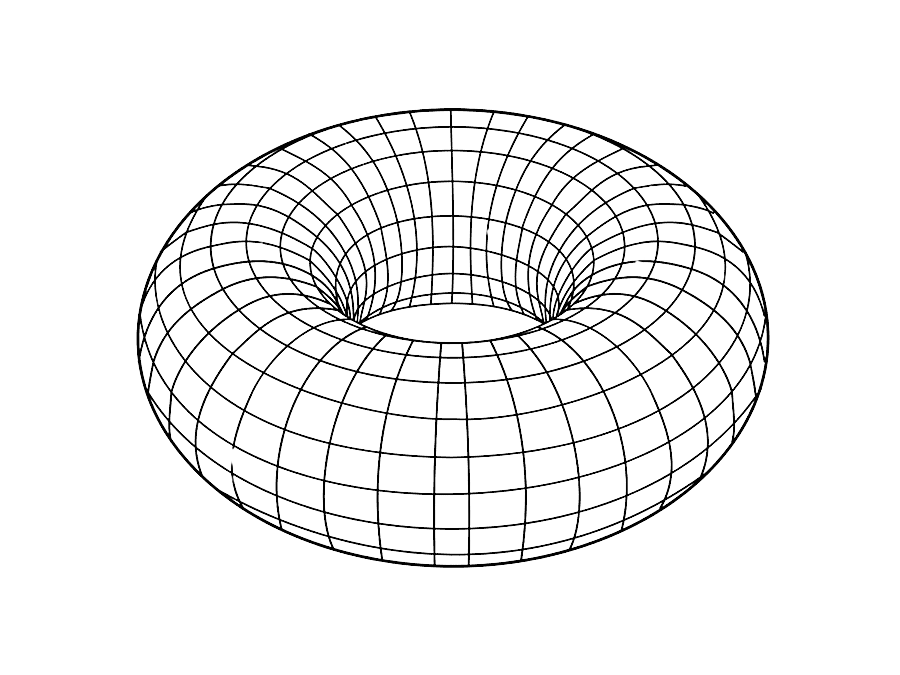
\includegraphics[width=0.6\linewidth]{figures/torus.png}
        \caption{Minh hoa cho hình Torus}
        \label{fig:torus}
    \end{figure}
    
\end{exercise}

\begin{exercise}
    Một bể bơi có hình dạng và kích thước như trong hình vẽ (đơn vị là mét). Bể bơi dài 20m, rộng 10m. Mực nước sâu 1m ở đầu cạn và 3m ở đầu sâu, với đáy dốc đều. Nếu bể chứa đầy nước, hãy tính công cần thiết để bơm hết nước ra khỏi thành bể.
\end{exercise}

\subsubsection{Ứng dụng trong vật lý}

\begin{exercise}
    Một chiếc xe đang di chuyển trên đường thẳng với vận tốc 88 ft/s thì người lái xe đạp phanh gấp. Xe giảm tốc với gia tốc không đổi là 11 ft/s$^2$.
    \begin{enumerate}[label=(\alph*)]
        \item Viết công thức cho vận tốc của xe sau $t$ giây kể từ lúc đạp phanh. Sau bao lâu thì xe dừng hẳn?
        \item Viết công thức cho quãng đường xe đi được sau $t$ giây kể từ lúc đạp phanh. Tính quãng đường xe đi được cho đến khi dừng hẳn.
    \end{enumerate}
\end{exercise}

\begin{exercise}
    Một dây cáp đồng nhất dài 10 mét và nặng 50 kg được treo thẳng đứng. Tính công cần thiết để kéo toàn bộ dây cáp lên đỉnh.
\end{exercise}

\begin{exercise}
    Một bể chứa nước hình bán cầu với bán kính 5 mét đang chứa đầy nước. Tính công cần thiết để bơm toàn bộ nước ra khỏi miệng bể. (Khối lượng riêng của nước là $\rho = 1000$ kg/m$^3$).
\end{exercise}

\begin{exercise}
    Theo định luật vạn vật hấp dẫn của Newton, lực hấp dẫn giữa hai vật có khối lượng $m_1$ và $m_2$ là $F = G \frac{m_1 m_2}{r^2}$, trong đó $r$ là khoảng cách giữa hai vật và $G$ là hằng số hấp dẫn.
    \begin{enumerate}[label=(\alph*)]
        \item Giả sử một trong hai vật được giữ cố định. Tính công cần thiết để di chuyển vật còn lại từ vị trí $r=a$ đến $r=b$.
        \item Tính công (năng lượng) cần thiết để phóng một tàu vũ trụ nặng 2000 kg từ bề mặt Trái Đất ra khỏi trường hấp dẫn của nó (tức là đến vô cùng).
    \end{enumerate}
    Giả sử khối lượng Trái Đất là $5.98 \times 10^{24}$ kg, bán kính Trái Đất là $6.37 \times 10^6$ m, và $G = 6.67 \times 10^{-11}$ N$\cdot$m$^2$/kg$^2$.
\end{exercise}

\begin{exercise}
    Dòng điện xoay chiều trong một mạch điện gia dụng có điện thế thay đổi theo phương trình $E(t) = A \sin(\omega t)$, trong đó $A$ là biên độ điện thế, $\omega$ là tần số góc. Các vôn kế đo \textbf{điện thế hiệu dụng} ($V_{rms}$), được định nghĩa là căn bậc hai của giá trị trung bình của $[E(t)]^2$ trong một chu kỳ.
    \[ V_{rms} = \sqrt{\frac{1}{T} \int_0^T [E(t)]^2 \dd t}. \]
    \begin{enumerate}[label=(\alph*)]
        \item Chứng minh rằng $V_{rms} = \frac{A}{\sqrt{2}}$.
        \item Một dòng điện gia dụng ở Việt Nam có điện thế hiệu dụng là 220V. Tìm biên độ điện thế $A$ của dòng điện này.
    \end{enumerate}
\end{exercise}

\begin{exercise}
    Một lò xo tuân theo định luật Hooke, tức là lực cần thiết để giữ lò xo bị kéo dãn một đoạn $x$ so với vị trí cân bằng là $F = kx$, trong đó $k$ là hằng số lò xo.
    \begin{enumerate}[label=(\alph*)]
        \item Nếu cần một lực 40 N để giữ một lò xo bị kéo dãn 10 cm, hãy tính công cần thiết để kéo dãn lò xo từ vị trí cân bằng đến 15 cm.
        \item Tính công cần thiết để kéo dãn lò xo thêm 5 cm nữa (từ 15 cm đến 20 cm).
    \end{enumerate}
\end{exercise}

\subsubsection{Ứng dụng trong kinh tế}

\begin{exercise}
    Hàm chi phí biên (marginal cost) để sản xuất $x$ đơn vị sản phẩm được cho bởi $C'(x) = 0.003x^2 - 0.8x + 75$. Chi phí cố định là $C(0) = 4000$.
    \begin{enumerate}[label=(\alph*)]
        \item Tìm hàm chi phí $C(x)$.
        \item Tính chi phí trung bình để sản xuất từ 100 đến 200 đơn vị sản phẩm.
    \end{enumerate}
\end{exercise}

\begin{exercise}
    Hàm doanh thu biên (marginal revenue) từ việc bán $q$ sản phẩm là $R'(q) = 450 - 0.8q$. Biết rằng không có doanh thu khi không có sản phẩm nào được bán.
    \begin{enumerate}[label=(\alph*)]
        \item Tìm hàm doanh thu $R(q)$.
        \item Tìm hàm cầu (demand function) $p(q)$, là giá bán của mỗi sản phẩm.
    \end{enumerate}
\end{exercise}

\begin{exercise}
    Hàm cung ứng (supply function) cho một sản phẩm là $p = S(x) = 10 + 0.1x + 0.0005x^2$, trong đó $p$ là giá bán mỗi đơn vị và $x$ là số lượng sản phẩm được cung ứng.
    \begin{enumerate}[label=(\alph*)]
        \item Tìm giá trung bình của sản phẩm khi mức cung ứng nằm trong khoảng từ 0 đến 50 đơn vị.
        \item Tìm mức cung ứng $x_0$ sao cho giá trung bình trong khoảng $[0, x_0]$ bằng 20.
    \end{enumerate}
\end{exercise}

\begin{exercise}
    Một công ty sản xuất máy tính xách tay. Phương trình cầu cho sản phẩm là $p = 1200 - 1.5x$, và hàm chi phí là $C(x) = 400x + 5000$, với $0 \le x \le 500$.
    \begin{enumerate}[label=(\alph*)]
        \item Tìm hàm lợi nhuận $P(x)$.
        \item Vẽ đồ thị hàm lợi nhuận.
        \item Với quy mô sản xuất nào thì công ty bắt đầu có lãi?
        \item Tìm quy mô sản xuất để đạt lợi nhuận tối đa.
        \item Tìm lợi nhuận trung bình nếu công ty sản xuất trong khoảng từ 200 đến 300 máy.
        \item Giả sử chính phủ đánh thuế 50 đô la trên mỗi máy bán ra. Công ty nên đặt giá bán mới là bao nhiêu để tối đa hóa lợi nhuận?
    \end{enumerate}
\end{exercise}

\begin{exercise}
    Một mỏ dầu đang sản xuất dầu với tốc độ $P'(t) = 120e^{-0.05t}$, trong đó $P'(t)$ được tính bằng nghìn thùng mỗi năm, và $t$ là số năm kể từ bây giờ.
    \begin{enumerate}[label=(\alph*)]
        \item Tổng sản lượng dầu sẽ được khai thác trong 5 năm tới là bao nhiêu?
        \item Giả sử mỏ dầu sẽ cạn kiệt. Hãy ước tính tổng trữ lượng dầu của mỏ.
    \end{enumerate}
\end{exercise}

\begin{exercise}
    Dòng tiền (cash flow) của một dự án đầu tư được dự đoán là $f(t) = 2000\sqrt{t+1}$ (đô la mỗi năm) trong vòng 8 năm tới. Nếu lãi suất chiết khấu liên tục là 5\% mỗi năm, hãy tính giá trị hiện tại (present value) của dòng tiền này.
    (Gợi ý: Giá trị hiện tại của một dòng tiền $f(t)$ trong khoảng $[0, T]$ với lãi suất $r$ là $\int_0^T f(t)e^{-rt} \dd t$).
\end{exercise}

\subsubsection{Xác suất}

\begin{exercise}
    Một biến ngẫu nhiên liên tục $X$ có hàm mật độ xác suất dạng $f(x) = kx(4-x)$, với $0 \le x \le 4$ và $k$ là một hằng số.
    \begin{enumerate}[label=(\alph*)]
        \item Tìm giá trị của hằng số $k$ để $f(x)$ là một hàm mật độ xác suất.
        \item Vẽ đồ thị của hàm mật độ xác suất $f(x)$.
        \item Tìm xác suất để biến ngẫu nhiên $X$ có giá trị nằm trong khoảng $[1, 2]$.
        \item Tìm xác suất để biến ngẫu nhiên $X$ có giá trị lớn hơn 3.
        \item Tính giá trị trung bình (kỳ vọng) của biến ngẫu nhiên này.
    \end{enumerate}
\end{exercise}

\begin{exercise}
    Tuổi thọ của một loại linh kiện điện tử (tính bằng giờ) được cho bởi hàm mật độ xác suất $f(x) = 0.001e^{-0.001x}$ với $x \ge 0$.
    \begin{enumerate}[label=(\alph*)]
        \item Vẽ đồ thị của hàm mật độ xác suất.
        \item Hãy kiểm tra rằng $f(x)$ thỏa mãn yêu cầu của một hàm mật độ xác suất.
        \item Tìm xác suất để một linh kiện hoạt động được ít nhất 500 giờ.
        \item Tìm xác suất để một linh kiện hỏng trong vòng 200 giờ đầu tiên.
        \item Tính tuổi thọ trung bình của loại linh kiện này.
    \end{enumerate}
\end{exercise}

\begin{exercise}
    Giả sử chiều cao của nam giới trưởng thành tại một quốc gia tuân theo phân phối chuẩn với giá trị trung bình là 175 cm và độ lệch chuẩn là 7 cm.
    \begin{enumerate}[label=(\alph*)]
        \item Viết công thức hàm mật độ xác suất cho biến ngẫu nhiên này.
        \item Tìm xác suất để một người đàn ông được chọn ngẫu nhiên có chiều cao từ 170 cm đến 180 cm. (Sử dụng máy tính để tính tích phân).
        \item Nếu một câu lạc bộ bóng rổ chỉ tuyển những người cao trên 190 cm, hãy ước tính tỉ lệ phần trăm nam giới trưởng thành đủ điều kiện tham gia.
    \end{enumerate}
\end{exercise}

\begin{exercise}
    Thời gian chờ xe buýt tại một trạm (tính bằng phút) là một biến ngẫu nhiên phân phối đều trên khoảng $[0, 15]$. Hàm mật độ xác suất là $f(x) = 1/15$ với $0 \le x \le 15$.
    \begin{enumerate}[label=(\alph*)]
        \item Tìm xác suất để một hành khách phải chờ từ 5 đến 10 phút.
        \item Tìm xác suất để hành khách phải chờ ít hơn 3 phút.
        \item Tính thời gian chờ trung bình.
    \end{enumerate}
\end{exercise}

\subsubsection{Các bài toán khác}

\begin{exercise}
    Nhiệt độ trong một ngày ở sa mạc có thể được mô hình hóa bởi hàm số $T(t) = 35 + 15\cos\left(\frac{\pi}{12}(t-4)\right)$, trong đó $t$ là số giờ kể từ nửa đêm. Tìm nhiệt độ trung bình trong khoảng thời gian từ 6 giờ sáng ($t=6$) đến 6 giờ tối ($t=18$).
\end{exercise}

\begin{exercise}
    Nồng độ của một loại thuốc trong máu của bệnh nhân sau $t$ giờ kể từ khi tiêm được mô hình hóa bởi hàm số $C(t) = 10te^{-0.5t}$ (mg/L).
    \begin{enumerate}[label=(\alph*)]
        \item Tính nồng độ trung bình của thuốc trong máu trong 4 giờ đầu tiên.
        \item Sử dụng máy tính để vẽ đồ thị hàm nồng độ. Tại thời điểm nào nồng độ thuốc đạt cực đại?
    \end{enumerate}
\end{exercise}

\begin{exercise}
    Ta đi từ nhà đến trường, một quãng đường dài 5 km, và mất tổng cộng 15 phút (0.25 giờ). Vận tốc trung bình của cả chuyến đi là $5 / 0.25 = 20$ km/h. Hãy giải thích tại sao chắc chắn phải có một thời điểm trong chuyến đi mà vận tốc tức thời của ta đúng bằng 20 km/h. (Gợi ý: Sử dụng Định lý Giá trị Trung bình cho Tích phân hoặc Định lý Giá trị Trung bình cho Đạo hàm).
\end{exercise}

\begin{exercise}
    Số lượng người (tính bằng nghìn người) đến một công viên giải trí trong một ngày được mô hình hóa bởi tốc độ $r(t) = 2 - 2\cos\left(\frac{\pi}{6}t\right)$, trong đó $t$ là số giờ kể từ lúc công viên mở cửa lúc 8 giờ sáng ($t=0$).
    \begin{enumerate}[label=(\alph*)]
        \item Công viên mở cửa trong 12 giờ. Tính tổng số lượt khách trong ngày.
        \item Tính số lượt khách trung bình mỗi giờ trong 4 giờ đầu tiên công viên mở cửa.
    \end{enumerate}
\end{exercise}

\begin{exercise}
    Lượng người đang bị mắc một bệnh truyền nhiễm (tính bằng nghìn người) vào thời điểm $t$ (tính bằng ngày kể từ khi dịch bùng phát) được mô hình hóa bởi hàm $N(t) = 25 t^2 e^{-t/5}$, với $0 \le t \le 40$.
    \begin{enumerate}[label=(\alph*)]
        \item Vẽ đồ thị của hàm số này bằng máy tính.
        \item Tìm thời điểm mà số người đang nhiễm bệnh đạt cực đại.
        \item Khi nào thì số người đang nhiễm bệnh bắt đầu giảm?
        \item Khi nào thì tốc độ lây nhiễm bắt đầu chậm lại (tức là tìm điểm uốn của đồ thị)?
        \item Tính số lượng người bệnh trung bình trong 20 ngày đầu tiên của đợt dịch.
    \end{enumerate}
\end{exercise}

\begin{exercise}
    Một nhà sinh thái học mô hình hóa quần thể của một loài cá trong hồ bằng phương trình logistic. Tốc độ tăng trưởng của quần thể được cho bởi $\frac{dP}{dt} = 0.2P\left(1 - \frac{P}{5000}\right)$, trong đó $P(t)$ là số lượng cá tại thời điểm $t$ (tính bằng năm).
    \begin{enumerate}[label=(\alph*)]
        \item Tốc độ tăng trưởng của quần thể lớn nhất khi nào? (Gợi ý: Tìm cực đại của hàm $\frac{dP}{dt}$).
        \item Nếu $P(0) = 1000$, hãy giải phương trình vi phân này để tìm $P(t)$. (Đây là một bài toán nâng cao, có thể tham khảo thêm sách về phương trình vi phân).
    \end{enumerate}
\end{exercise}
